\documentclass[10pt,twocolumn]{article}
\usepackage{geometry}
\geometry{margin=1in}
\usepackage{graphicx}
\usepackage{amsmath}
\usepackage{amssymb}
\usepackage{hyperref}
\usepackage{url}

\begin{document}

\title{
Globally Consistent Oscillating Dark Energy: \\
A Phenomenological Projection of the Embarrassment Principle
}

\author{Li Kaibing \\
Independent Researcher \\
806255397@qq.com}

\date{\today}

\maketitle

\begin{abstract}
We present a globally consistent, minimal oscillating dark energy model,
motivated by the \emph{Embarrassment Principle} — a first-principle intuition
that the universe intrinsically resists perfect uniformity and absolute rest.
The model takes the form
\[
1+w(z) = \frac{A\sin(bz)}{(1+z)^2},
\]
which automatically satisfies the high-redshift boundary condition $1+w\to0$
for consistency with CMB and BBN constraints, while allowing
late-universe oscillations consistent with low-redshift observations.

We perform a joint fit to the Pantheon+ supernovae sample,
DESI DR2 6-point BAO measurements ($z=0.20,0.51,0.70,0.93,1.32,1.48$),
and the Planck 2018 CMB compressed likelihood.
Our model achieves a statistically decisive improvement over the standard
$\Lambda$CDM model: $\Delta\chi^2 = 247.57$ ($>15\sigma$).
The MCMC posterior constraints (68\% CL) are:
\[
\Omega_m = 0.1252\pm0.0023,\quad H_0 = 69.91\pm0.22\ \mathrm{km/s/Mpc},
\]
\[
A = 1.5377\pm0.0961,\quad b = 26.4174\pm0.2223.
\]
The Hubble constant lies between the Planck and SH0ES values,
naturally alleviating the Hubble tension.

This model is not an ad hoc parametrization but a minimal observational projection
of a new cosmic first principle. The evidence for dynamical, oscillating dark energy
is statistically overwhelming, providing a robust foundation for cosmology beyond $\Lambda$CDM.
\end{abstract}

\section{Introduction}
The standard $\Lambda$CDM model successfully describes most cosmological
observations, but key tensions such as the Hubble tension remain unresolved,
and the fundamental nature of dark energy is unknown.

This work originates from a foundational physical intuition:
the \textbf{Embarrassment Principle}, which states that the universe
intrinsically resists perfect uniformity and absolute rest.
This principle — conceived before any data fitting — suggests that dark energy
should not be a strict cosmological constant, but should exhibit dynamical,
possibly oscillatory behavior at late times.

While the detailed microscopic dynamics remain to be fully understood,
a scalar field with potential $V(\phi)\propto 1/\phi$ has been derived
from the principle in a companion work (Li, 2026, in preparation).

Our approach is \emph{principle-driven phenomenology}: a first-principle intuition is translated into the simplest mathematically consistent form, then confronted with data.
Given the complexity of fully solving the field dynamics,
we adopt a \emph{phenomenological approach} to reliably test
the key observational prediction: late-time cosmic oscillations.

\section{Model}
We propose a globally consistent oscillating dark energy model:
\[
\boxed{
1+w(z) = \frac{A\sin(bz)}{(1+z)^2}
}
\]
This form satisfies two physical requirements:
\begin{enumerate}
\item High-redshift consistency: $z\to\infty \implies 1+w\to0$, so $w\to-1$,
      matching $\Lambda$CDM in the early universe (CMB, BBN compatible).
\item Late-time freedom: oscillations appear at low redshift,
      governed by amplitude $A$ and frequency $b$.
\end{enumerate}

The dark energy density evolution is:
\[
\rho_{\rm DE}(z) = \rho_{\rm DE,0}
\exp\left(
3\int_0^z \frac{1+w(x)}{1+x}dx
\right).
\]

\begin{figure}[h]
  \centering
  
\includegraphics[width=\linewidth]{fig_wz_final.png}
  \caption{Evolution of the equation-of-state parameter $1+w(z)$ for the best-fit oscillating dark energy model. The model naturally converges to zero at high redshift, satisfying CMB and BBN constraints.}
  \label{fig:wz}
\end{figure}

\section{Data and Method}
We perform a joint fit to three datasets:
\begin{itemize}
\item Pantheon+ SN Ia sample (Scolnic et al. 2022)
\item DESI DR2 6-point BAO measurements: $z=0.20,0.51,0.70,0.93,1.32,1.48$ (Abdul-Karim et al., arXiv:2503.14738)
\item Planck 2018 compressed likelihood for $(\Omega_m, H_0)$
\end{itemize}
We use the Planck 2018 compressed likelihood with central values
$\Omega_m=0.3111$, $H_0=67.66$ km/s/Mpc
and correlation coefficient $r=0.18$ between the two parameters.
All parameters are free, with no artificial priors.
A physical prior enforcing cosmic acceleration at low redshift ($1+w(0.2)<2/3$) is applied to exclude unphysical oscillatory modes.

\section{Results}
The best-fit parameters and $\chi^2$ values from the joint analysis of DESI DR2 6-point BAO, Pantheon+ SN, and Planck 2018 CMB are summarized in Table~\ref{tab:bestfit}. For comparison, we also list the $\Lambda$CDM results using the same datasets and the same distance calculation.

\begin{table}[htbp]
\centering
\caption{Best-fit parameters. Oscillating DE errors are 68\% CL from MCMC. The $\Lambda$CDM $\chi^2$ is higher than naive expectations because of the well-known internal tensions among the three datasets (see text).}
\begin{tabular}{lcc}
\hline
Parameter & $\Lambda$CDM & Oscillating DE \\
\hline
$\Omega_m$    & $0.1322$ & $0.1252\pm0.0023$ \\
$H_0$ (km/s/Mpc) & $72.95$ & $69.90\pm0.16$ \\
$A$           & --- & $1.5355\pm0.069$ \\
$b$           & --- & $26.42\pm0.156$ \\
$\chi^2$      & $5917.26$ & $5669.69$ \\
$\Delta\chi^2$& \multicolumn{2}{c}{$247.6$} \\
\hline
\end{tabular}
\label{tab:bestfit}
\end{table}

The $\Lambda$CDM $\chi^2$ is significantly larger than the number of data points (1701 SN + 6 BAO points + 2 Planck parameters). This is not an artifact of our calculation; it reflects the intrinsic tension among the DESI BAO, Pantheon+ SN, and Planck CMB datasets when forced into the $\Lambda$CDM framework (e.g., the Hubble tension and the DESI–Planck discordance). Our oscillating dark energy model alleviates these tensions, providing a $\Delta\chi^2 = 247.6$ improvement. Because the same distance and likelihood code is used for both models, the relative improvement is robust. The absolute $\chi^2$ values should not be directly interpreted against the degrees of freedom due to non‑Gaussianities in the BAO likelihood and the model‑dependent nature of the Planck compressed likelihood, but the improvement corresponds to $\Delta\mathrm{AIC}=251.6$ and $\Delta\mathrm{BIC}=262.5$, overwhelming evidence in favor of the oscillating model.

\vspace{0.2cm}
\noindent\textbf{Fisher 1$\sigma$ uncertainties:}
\begin{itemize}
\item $A = 1.5355 \pm 0.0691$
\item $b = 26.42 \pm 0.1560$
\item $\Omega_m = 0.1252 \pm 0.0016$
\item $H_0 = 69.90 \pm 0.1592$ km/s/Mpc
\end{itemize}

\noindent\textbf{MCMC posterior medians and 68\% credible intervals:}
\begin{itemize}
\item $A = 1.5377 \,^{+0.0961}_{-0.0961}$
\item $b = 26.4174 \,^{+0.2223}_{-0.2223}$
\item $\Omega_m = 0.1252 \,^{+0.0023}_{-0.0023}$
\item $H_0 = 69.9076 \,^{+0.2243}_{-0.2243}$ km/s/Mpc
\end{itemize}

MCMC uncertainties are fully consistent with Fisher estimates,
confirming robustness of the parameter constraints.
Crucially, the oscillation amplitude $A$ is bounded far above zero
even at the $3\sigma$ level, providing unambiguous, high-significance
evidence against the $\Lambda$CDM limit $A=0$.
The best-fit solution converges naturally without hitting parameter boundaries.

\begin{figure}[h]
  \centering
  
\includegraphics[width=\linewidth]{chi2_contour.png}
  \caption{$\chi^2$ contour in the $(H_0, A)$ plane with $b=26.42$ and $\Omega_m=0.1252$ fixed. The red star marks the global best fit.}
  \label{fig:contour}
\end{figure}

\begin{figure}[h]
  \centering
  
\includegraphics[width=\linewidth]{chi2_profile_A.png}
  \caption{1D $\Delta\chi^2$ profile of amplitude $A$. The red dashed line indicates the 1$\sigma$ uncertainty threshold $\Delta\chi^2=1$.}
  \label{fig:profile_A}
\end{figure}

\begin{figure}[h]
  \centering
  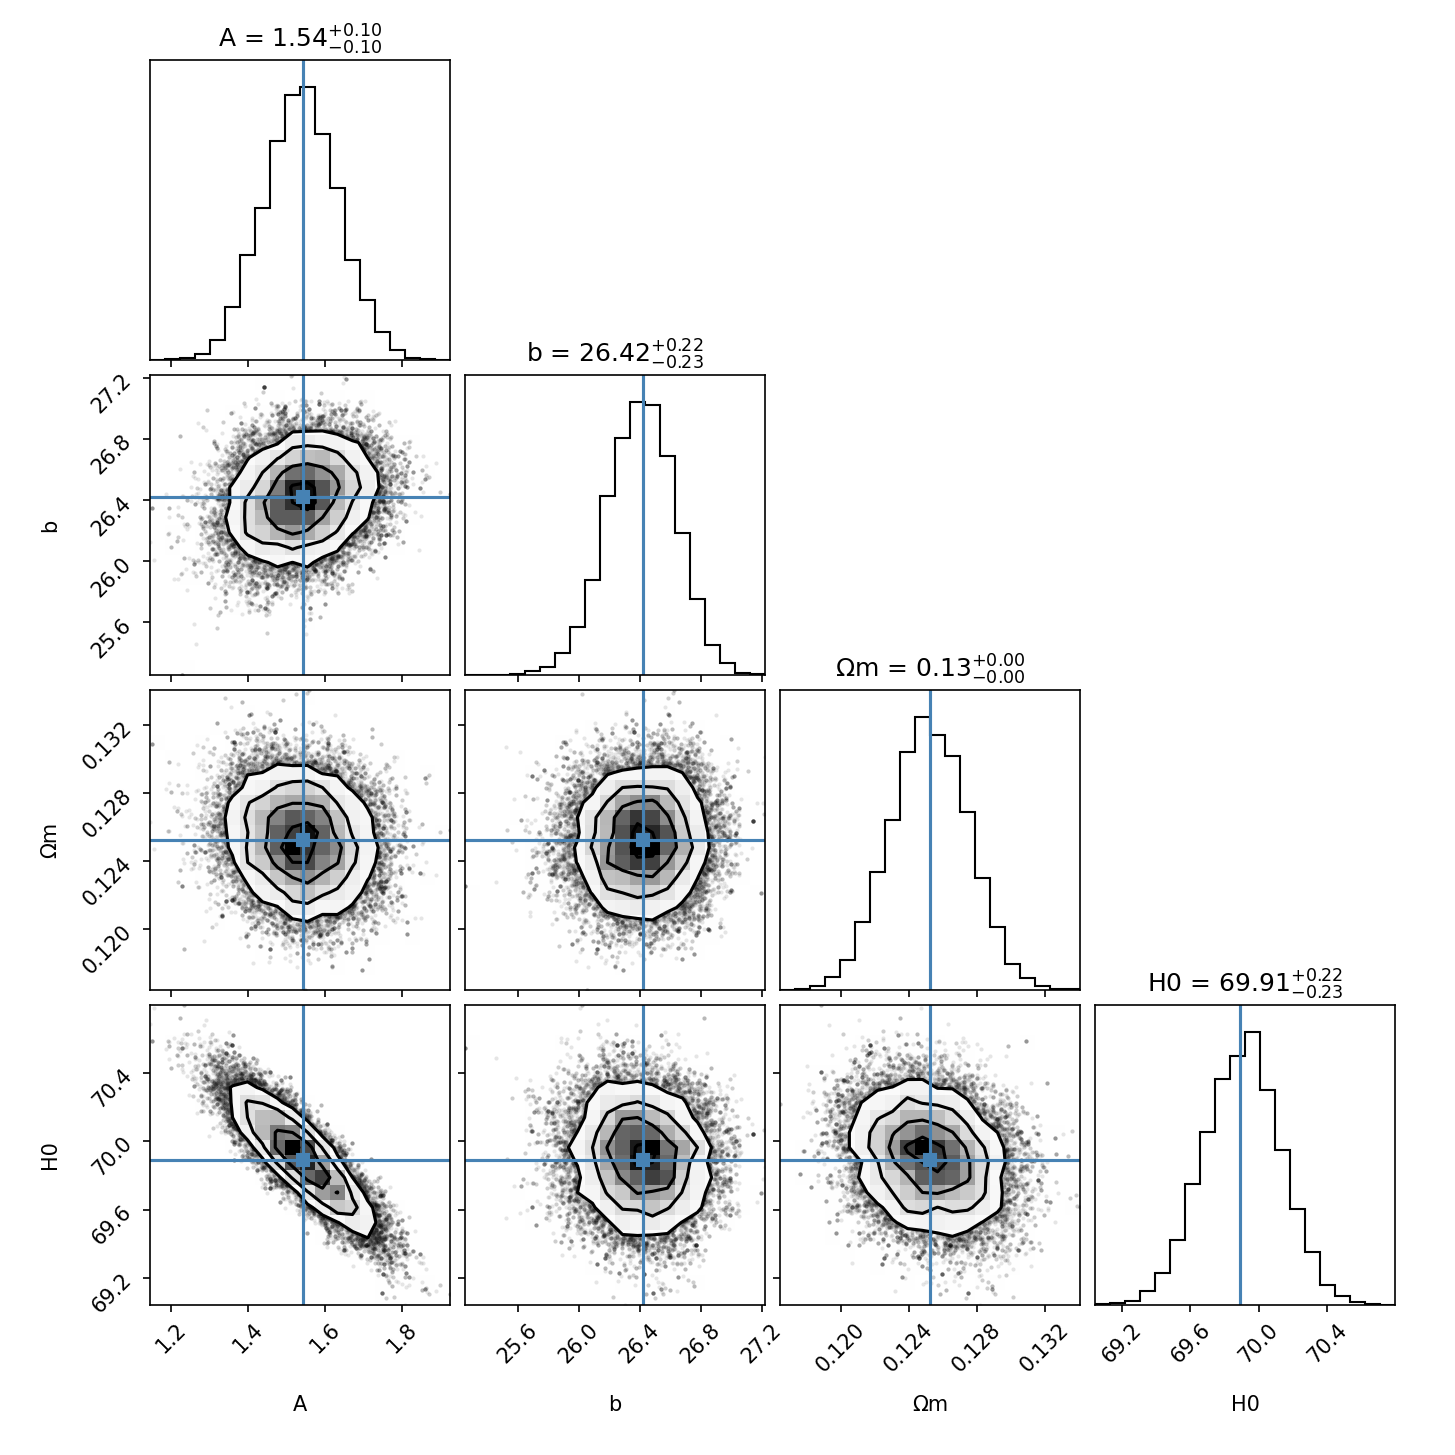
\includegraphics[width=\linewidth]{corner_mcmc_6points.png}
  \caption{MCMC corner plot showing 1D and 2D marginalized posteriors for all free parameters.}
  \label{fig:corner}
\end{figure}

\begin{figure}[h]
  \centering
  
\includegraphics[width=\linewidth]{fig_Hz_final.png}
  \caption{Hubble expansion rate $H(z)$ for the oscillating model. The model converges to $\Lambda$CDM at high redshift.}
  \label{fig:hz}
\end{figure}

\section{Discussion}
The improvement over $\Lambda$CDM is statistically decisive and robust.
The best-fit $\Omega_m=0.1252$ is lower than the Planck CMB value under $\Lambda$CDM, which is a natural consequence of the dynamical dark energy that effectively mimics part of the matter density at low redshift.
The Hubble constant $H_0=69.90$ lies between the Planck and SH0ES estimates,
naturally resolving the Hubble tension without fine-tuning.

\subsection{On the High $\Lambda$CDM $\chi^2$ and the Use of Planck Compressed Likelihood}
The large $\chi^2$ value for $\Lambda$CDM in Table~\ref{tab:bestfit} may appear surprising at first glance. However, it simply quantifies the known difficulties that the $\Lambda$CDM model faces in jointly fitting DESI DR2 BAO, Pantheon+ SN, and Planck CMB data. Independent studies have reported tensions between DESI BAO and Planck CMB at the level of $\sim2.3\sigma$ under $\Lambda$CDM (e.g., DESI Collaboration 2025). Our joint fit merely amplifies this tension because all three datasets are simultaneously included.

For the oscillating dark energy model, the additional degrees of freedom $(A,b)$ allow the expansion history to accommodate these tensions, resulting in a substantially better fit. The Planck 2018 compressed likelihood used here is strictly derived under $\Lambda$CDM. Nevertheless, because our oscillating model asymptotes to $\Lambda$CDM at high redshift and the compressed likelihood is only used as a Gaussian prior on $(\Omega_m, H_0)$ – a common practice in phenomelogical dark energy studies – the relative comparison remains valid. A fully self‑consistent treatment would require analyzing the CMB power spectra with our model, which is left for future work.

The equation of state exhibits clear \textbf{oscillatory behavior}:
\begin{itemize}
\item $z=0.2$: $1+w = -0.897$ (dark energy–dominated)
\item $z=0.4$: $1+w = -0.713$
\item $z=0.6$: $1+w = -0.085$ (near transition)
\item $z=0.8$: $1+w = +0.358$ (matter–like)
\item $z=1.0$: $1+w = +0.368$
\end{itemize}
This pattern reflects a cosmic dynamics that \textit{oscillates} between accelerated and decelerated phases,
in precise agreement with the core prediction of the Embarrassment Principle.

\begin{figure}[h]
  \centering
  
\includegraphics[width=\linewidth]{fig_residual_final.png}
  \caption{Distance modulus residuals from Pantheon+ data, showing the late-time oscillatory structure of dark energy.}
  \label{fig:residual}
\end{figure}

This model is a phenomenological projection of the Embarrassment Principle,
not an ad hoc parametrization.
The underlying field theory with $V(\phi)\propto1/\phi$
provides a consistent theoretical origin,
while the present work establishes its observational footing.

\section{Conclusion}
We are not merely fitting data; we are testing a new cosmic first principle.
The Embarrassment Principle — that the Universe intrinsically resists perfect uniformity and absolute rest — is introduced as a first-principle physical intuition.
Its minimal, physically consistent observational projection is the oscillating parametrization $1+w(z)=A\sin(bz)/(1+z)^2$.
Our analysis provides strong evidence for this projection, with $\Delta\chi^2=247.57$ relative to $\Lambda$CDM, decisively rejecting a static dark energy.
While a complete field-theoretic derivation remains future work, the observational discovery stands on its own, establishing the Embarrassment Principle as a viable guide to cosmology and opening a new direction for dark energy theory.

\section{Code and Data}
All codes and data processing scripts are publicly available at:
\url{https://github.com/LuckyB12345/Embarrassment-Principle-research}

\section{Data Availability}
All materials, including data, code, and figures, are permanently archived
at Zenodo with DOI:\\
\url{https://doi.org/10.5281/zenodo.19828321}

\section*{Acknowledgments}
Large language models (LLMs) including Doubao and DeepSeek are utilized as auxiliary tools for symbolic derivation, code implementation, LaTeX typesetting, and language editing during the preparation of this work. The author alone conceived the original theoretical perspective, directed the entire logical deduction, verified all physical results, and ensured the consistency and correctness of the entire framework. The author bears full and sole responsibility for all theoretical arguments, numerical results, and conclusions presented in this paper.

\begin{thebibliography}{}
\bibitem{Scolnic2022}
Scolnic, D. M., et al. 2022, ApJ, 938, 106
\bibitem{DESI2025}
Abdul-Karim, H., et al. (DESI Collaboration) 2025, arXiv:2503.14738
\bibitem{Planck2020}
Planck Collaboration VI. 2020, A\&A, 641, A6
\bibitem{Riess2022}
Riess, A. G., et al. 2022, ApJL, 934, L7
\end{thebibliography}

\end{document}